%%%%%%%%%%%%%%%%%%%%%%%%%%%%%%%%%%%%%%%%%
% baposter Portrait Poster
% LaTeX Template
% Version 1.0 (15/5/13)
%
% Created by:
% Brian Amberg (baposter@brian-amberg.de)
%
% This template has been downloaded from:
% http://www.LaTeXTemplates.com
%
% License:
% CC BY-NC-SA 3.0 (http://creativecommons.org/licenses/by-nc-sa/3.0/)
%
%%%%%%%%%%%%%%%%%%%%%%%%%%%%%%%%%%%%%%%%%

%----------------------------------------------------------------------------------------
%	PACKAGES AND OTHER DOCUMENT CONFIGURATIONS
%----------------------------------------------------------------------------------------

\documentclass[archE1,portrait]{baposter}

%841mm x 1189mm
\usepackage[font=small,labelfont=bf]{caption} % Required for specifying captions to tables and figures
\usepackage{booktabs} % Horizontal rules in tables
\usepackage{relsize} % Used for making text smaller in some places
\usepackage[urlcolor  = blue]{hyperref}
\usepackage{float}
\graphicspath{{figures/}} % Directory in which figures are stored

\definecolor{bordercol}{RGB}{5,2,82} % Border color of content boxes
\definecolor{headercol1}{RGB}{5,2,82} % Background color for the header in the content boxes (left side)
\definecolor{headercol2}{RGB}{5,2,82} % Background color for the header in the content boxes (right side)
\definecolor{headerfontcol}{RGB}{255,255,255} % Text color for the header text in the content boxes
\definecolor{boxcolor}{RGB}{255,255,255} % Background color for the content in the content boxes

\begin{document}

\background{ % Set the background to an image (background.pdf)

}

\begin{poster}{
grid=false,
borderColor=bordercol, % Border color of content boxes
headerColorOne=headercol1, % Background color for the header in the content boxes (left side)
headerColorTwo=headercol1, % Background color for the header in the content boxes (right side)
headerFontColor=headerfontcol, % Text color for the header text in the content boxes
boxColorOne=boxcolor, % Background color for the content in the content boxes
headershape=roundedright, % Specify the rounded corner in the content box headers
headerfont=\Large\sf\bf, % Font modifiers for the text in the content box headers
textborder=rectangle,
background=user,
headerborder=open, % Change to closed for a line under the content box headers
boxshade=plain,
columns=4
}
{}
%
%----------------------------------------------------------------------------------------
%	TITLE AND AUTHOR NAME
%----------------------------------------------------------------------------------------
%
%\vspace{2em}
{
%\newline
\sf\bf Temporal properties of social networks} % Poster title
{
\vspace{1em} {\LARGE\bf \underline{Team 18}}\\
%\vspace{1em}
Rik Schreurs, Francois van der Ven, Loek Tonnaer\\ % Author names
{\smaller \{h.c.m.scheurs, f.v.d.ven, l.m.a.tonnaer\}@student.tue.nl}\\
\vspace{1em}
} % Author email addresses
%

%----------------------------------------------------------------------------------------
%	DATA
%----------------------------------------------------------------------------------------

\headerbox{Data}{name=introduction,column=0,row=0, span=2}{
\begin{itemize}
\item Edge data from three social networks, connections between users
\end{itemize}

\begin{center}
\begin{tabular}{l|l|l|l|l}
            & Facebook & YouTube   & Flickr     &  \\ \cline{1-4}
\# edges    & 817.037  & 9.375.374 & 33.140.017 &  \\ \cline{1-4}
\# vertices & 63.731   & 3.223.589 & 2.302.925  &  \\ \cline{1-4}
Size        & 15,5 MB  & 257,1 MB  & 901,5 MB   &  \\ \cline{1-4}
\end{tabular}
\end{center}


\underline{\textbf{Programming setup}}
\begin{itemize}
\item \emph{Apache Flink}
\item Graph processing API and library: \emph{Gelly}
\end{itemize}
}

%\headerbox{True vs False Motifs}{name=introduction2,column=1,row=0, span=2}{
%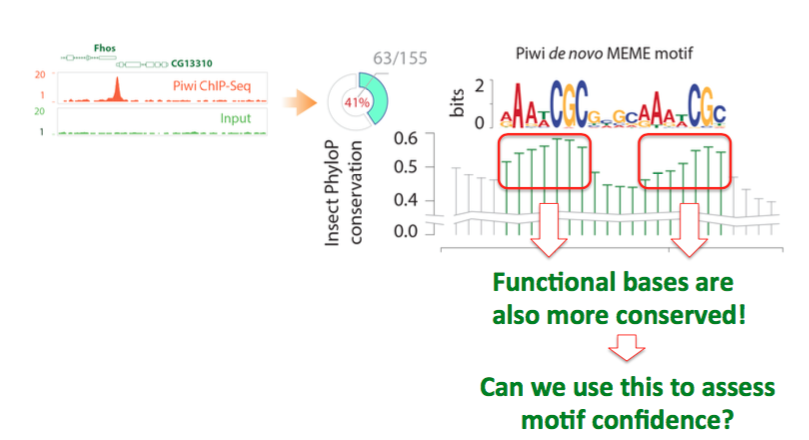
\includegraphics[scale=0.42]{motif_study}
%}

%----------------------------------------------------------------------------------------
%	OBJECTIVES
%----------------------------------------------------------------------------------------

\headerbox{Objectives}{name=methods,column=2,row=0,span=2}{


\underline{\textbf{Temporal aspects}}
\begin{itemize}
\item How long does it take for a new user to achieve a certain number of connections?
\item Degrees of separation, in how many steps can you go from one user to any other? How does this evolve over time?
\item How ``connected'' is each of the graphs? How many connected components are there, and how does this change over time?
\end{itemize}


}





%----------------------------------------------------------------------------------------
%	RESULTS
%----------------------------------------------------------------------------------------
\headerbox{Results}{name=results2,span=4,column=0,below=introduction}{
\begin{figure}[H]
\centering
% \begin{minipage}[b]{0.45\linewidth}
% 	\includegraphics[width=1\linewidth]{edges.png}
% \end{minipage}
% \quad
% \begin{minipage}[b]{0.45\linewidth}
% 	\includegraphics[width=1\linewidth]{std-dev.png}
% \end{minipage}

\begin{minipage}[b]{0.3\linewidth}
	\includegraphics[width=1\linewidth]{FacebookConnectedComponents.png}
\end{minipage}
\begin{minipage}[b]{0.3\linewidth}
	\includegraphics[width=1\linewidth]{YouTubeConnectedComponents.png}
\end{minipage}
\begin{minipage}[b]{0.3\linewidth}
	\includegraphics[width=1\linewidth]{FlickrConnectedComponents.png}
\end{minipage}

\end{figure}
}


%----------------------------------------------------------------------------------------
%	CONCLUSIONS
%----------------------------------------------------------------------------------------
\headerbox{Conclusions}{name=conclusion,span=4,column=0,below=results2}{
\begin{itemize}
\item Conclusion 1
\item Conclusion 2
\item Conclusion 3
\end{itemize}
}

%----------------------------------------------------------------------------------------
\vspace*{20em}

\includegraphics[width=0.3\textwidth]{tue-logo}

\end{poster}
\end{document}